% Options for packages loaded elsewhere
\PassOptionsToPackage{unicode}{hyperref}
\PassOptionsToPackage{hyphens}{url}
\PassOptionsToPackage{dvipsnames,svgnames,x11names}{xcolor}
%
\documentclass[
  11pt,
  a4paper,
]{tudscrreprt}

\usepackage{amsmath,amssymb}
\usepackage{setspace}
\usepackage{iftex}
\ifPDFTeX
  \usepackage[T1]{fontenc}
  \usepackage[utf8]{inputenc}
  \usepackage{textcomp} % provide euro and other symbols
\else % if luatex or xetex
  \usepackage{unicode-math}
  \defaultfontfeatures{Scale=MatchLowercase}
  \defaultfontfeatures[\rmfamily]{Ligatures=TeX,Scale=1}
\fi
\usepackage{lmodern}
\ifPDFTeX\else  
    % xetex/luatex font selection
\fi
% Use upquote if available, for straight quotes in verbatim environments
\IfFileExists{upquote.sty}{\usepackage{upquote}}{}
\IfFileExists{microtype.sty}{% use microtype if available
  \usepackage[]{microtype}
  \UseMicrotypeSet[protrusion]{basicmath} % disable protrusion for tt fonts
}{}
\makeatletter
\@ifundefined{KOMAClassName}{% if non-KOMA class
  \IfFileExists{parskip.sty}{%
    \usepackage{parskip}
  }{% else
    \setlength{\parindent}{0pt}
    \setlength{\parskip}{6pt plus 2pt minus 1pt}}
}{% if KOMA class
  \KOMAoptions{parskip=half}}
\makeatother
\usepackage{xcolor}
\setlength{\emergencystretch}{3em} % prevent overfull lines
\setcounter{secnumdepth}{5}
% Make \paragraph and \subparagraph free-standing
\ifx\paragraph\undefined\else
  \let\oldparagraph\paragraph
  \renewcommand{\paragraph}[1]{\oldparagraph{#1}\mbox{}}
\fi
\ifx\subparagraph\undefined\else
  \let\oldsubparagraph\subparagraph
  \renewcommand{\subparagraph}[1]{\oldsubparagraph{#1}\mbox{}}
\fi


\providecommand{\tightlist}{%
  \setlength{\itemsep}{0pt}\setlength{\parskip}{0pt}}\usepackage{longtable,booktabs,array}
\usepackage{calc} % for calculating minipage widths
% Correct order of tables after \paragraph or \subparagraph
\usepackage{etoolbox}
\makeatletter
\patchcmd\longtable{\par}{\if@noskipsec\mbox{}\fi\par}{}{}
\makeatother
% Allow footnotes in longtable head/foot
\IfFileExists{footnotehyper.sty}{\usepackage{footnotehyper}}{\usepackage{footnote}}
\makesavenoteenv{longtable}
\usepackage{graphicx}
\makeatletter
\def\maxwidth{\ifdim\Gin@nat@width>\linewidth\linewidth\else\Gin@nat@width\fi}
\def\maxheight{\ifdim\Gin@nat@height>\textheight\textheight\else\Gin@nat@height\fi}
\makeatother
% Scale images if necessary, so that they will not overflow the page
% margins by default, and it is still possible to overwrite the defaults
% using explicit options in \includegraphics[width, height, ...]{}
\setkeys{Gin}{width=\maxwidth,height=\maxheight,keepaspectratio}
% Set default figure placement to htbp
\makeatletter
\def\fps@figure{htbp}
\makeatother
% definitions for citeproc citations
\NewDocumentCommand\citeproctext{}{}
\NewDocumentCommand\citeproc{mm}{%
  \begingroup\def\citeproctext{#2}\cite{#1}\endgroup}
\makeatletter
 % allow citations to break across lines
 \let\@cite@ofmt\@firstofone
 % avoid brackets around text for \cite:
 \def\@biblabel#1{}
 \def\@cite#1#2{{#1\if@tempswa , #2\fi}}
\makeatother
\newlength{\cslhangindent}
\setlength{\cslhangindent}{1.5em}
\newlength{\csllabelwidth}
\setlength{\csllabelwidth}{3em}
\newenvironment{CSLReferences}[2] % #1 hanging-indent, #2 entry-spacing
 {\begin{list}{}{%
  \setlength{\itemindent}{0pt}
  \setlength{\leftmargin}{0pt}
  \setlength{\parsep}{0pt}
  % turn on hanging indent if param 1 is 1
  \ifodd #1
   \setlength{\leftmargin}{\cslhangindent}
   \setlength{\itemindent}{-1\cslhangindent}
  \fi
  % set entry spacing
  \setlength{\itemsep}{#2\baselineskip}}}
 {\end{list}}
\usepackage{calc}
\newcommand{\CSLBlock}[1]{\hfill\break\parbox[t]{\linewidth}{\strut\ignorespaces#1\strut}}
\newcommand{\CSLLeftMargin}[1]{\parbox[t]{\csllabelwidth}{\strut#1\strut}}
\newcommand{\CSLRightInline}[1]{\parbox[t]{\linewidth - \csllabelwidth}{\strut#1\strut}}
\newcommand{\CSLIndent}[1]{\hspace{\cslhangindent}#1}

\faculty{Fakultät Umweltwissenschaften}
\department{Fachrichtung Hydrowissenschaften}
\institute{Institut für Hydrobiologie}
\chair{Professur für Limnologie (Gewässerökologie)}
\course{M.Sc. Hydrobiologie}
\subject{Berufspraktikumsbericht} % Zeile bei Bachelor- und Masterarbeiten ändern oder löschen
\graduation[M.Sc.]{Master of Science}
% \dateofbirth{02.01.2001}  % Optional
% \placeofbirth{Dresden}    % Optional
\referee{Prof. Annegret Clearwater (TU Dresden)\and Dr. Michael Fischer (Umweltforschungszentrum)}
\supervisor{Dipl.-Biol. Luise Salomo, MSc. Axel Adam}
% \defensedate{10.09.2024}  % Optional
\makeatletter
\@ifpackageloaded{caption}{}{\usepackage{caption}}
\AtBeginDocument{%
\ifdefined\contentsname
  \renewcommand*\contentsname{Inhaltsverzeichnis}
\else
  \newcommand\contentsname{Inhaltsverzeichnis}
\fi
\ifdefined\listfigurename
  \renewcommand*\listfigurename{Abbildungsverzeichnis}
\else
  \newcommand\listfigurename{Abbildungsverzeichnis}
\fi
\ifdefined\listtablename
  \renewcommand*\listtablename{Tabellenverzeichnis}
\else
  \newcommand\listtablename{Tabellenverzeichnis}
\fi
\ifdefined\figurename
  \renewcommand*\figurename{Abbildung}
\else
  \newcommand\figurename{Abbildung}
\fi
\ifdefined\tablename
  \renewcommand*\tablename{Tabelle}
\else
  \newcommand\tablename{Tabelle}
\fi
}
\@ifpackageloaded{float}{}{\usepackage{float}}
\floatstyle{ruled}
\@ifundefined{c@chapter}{\newfloat{codelisting}{h}{lop}}{\newfloat{codelisting}{h}{lop}[chapter]}
\floatname{codelisting}{Listing}
\newcommand*\listoflistings{\listof{codelisting}{Listingverzeichnis}}
\makeatother
\makeatletter
\makeatother
\makeatletter
\@ifpackageloaded{caption}{}{\usepackage{caption}}
\@ifpackageloaded{subcaption}{}{\usepackage{subcaption}}
\makeatother
\ifLuaTeX
\usepackage[bidi=basic]{babel}
\else
\usepackage[bidi=default]{babel}
\fi
\babelprovide[main,import]{ngerman}
% get rid of language-specific shorthands (see #6817):
\let\LanguageShortHands\languageshorthands
\def\languageshorthands#1{}
\ifLuaTeX
  \usepackage{selnolig}  % disable illegal ligatures
\fi
\usepackage{bookmark}

\IfFileExists{xurl.sty}{\usepackage{xurl}}{} % add URL line breaks if available
\urlstyle{same} % disable monospaced font for URLs
\hypersetup{
  pdftitle={Entwicklung einer Universalmethode zur Umsetzung der Wasserrahmenrichtlinie},
  pdfauthor={Silke Musterfrau},
  pdflang={de},
  colorlinks=true,
  linkcolor={blue},
  filecolor={Maroon},
  citecolor={Blue},
  urlcolor={Blue},
  pdfcreator={LaTeX via pandoc}}

\title{Entwicklung einer Universalmethode zur Umsetzung der
Wasserrahmenrichtlinie}
\author{Silke Musterfrau}
\date{25. August 2024}

\begin{document}
\maketitle
\begin{abstract}
\textbf{Abstract:} The English abstract should briefly summarize task,
methods and main results. Lorem ipsum dolor sit amet, consetetur
sadipscing elitr, sed diam nonumy eirmod tempor invidunt ut labore et
dolore magna aliquyam erat, sed diam voluptua. At vero eos et accusam et
justo duo dolores et ea rebum.\\
\strut \\
\textbf{Zusammenfassung:} Die Zusammenfassung soll die Aufgabe, die
Methoden und die wichtigsten Ergebnisse kurz zusammenfassen. Lorem ipsum
dolor sit amet, consetetur sadipscing elitr, sed diam nonumy eirmod
tempor invidunt ut labore et dolore magna aliquyam erat, sed diam
voluptua. At vero eos et accusam et justo duo dolores et ea rebum.
\end{abstract}

\renewcommand*\contentsname{Inhaltsverzeichnis}
{
\hypersetup{linkcolor=}
\setcounter{tocdepth}{2}
\tableofcontents
}
\listoffigures
\listoftables
\setstretch{1.2}
\faculty{Fakultät Umweltwissenschaften}
\department{Fachrichtung Hydrowissenschaften}
\institute{Institut für Hydrobiologie}
\chair{Professur für Limnologie (Gewässerökologie)}

\chapter{Einleitung}\label{einleitung}

In der Einleitung beschreibt man zunächst den bekannten Kontext. Danach
stellt man das zu lösende Problem dar. Es ist sehr wichtig, die
wissenschaftliche oder methodische Fragstellung klar herauszuarbeiten.
Falls möglich, sollte die Fragestellung als Hypothese formuliert werden.
Anschließend leitet man ab, wie das Problem gelöst werden soll.

\section{Stand der Technik}\label{stand-der-technik}

Quarto (RStudio Team, 2024) ist ein Textsatzsystem bei dem man Code
verschiedener Skriptsprachen direkt einbetten kann, z.B. R (R Core Team,
2024), Python oder Julia. Dies ermöglicht es, Berechnungen und
statistische Analysen direkt im Textdokument durchführen zu lassen und
Grafiken direkt an Ort und Stelle zu erzeugen.

Der Output kann in HTML, Word, oder als PDF erfolgen. Hierbei bietet es
sich an, zunächst mit HTML zu arbeiten, weil dies schneller und
unkomplizierter funktioniert. Für die Endversion benutzt man dann Word
oder PDF.

\section{Zielstellung}\label{zielstellung}

Es sollte eine Formatvorlage in Quarto erstellt werden, aus der mit
Hilfe des Latex-Systems (Lamport, 2005) ein PDF erzeugt werden kann. Als
Basis sollte das Corporate Design der TU Dresden in Form eines
Vorhandenen Latex-Klasse verwendet werden. Das Ergebnis soll möglichst
professionell aussehen, allerdings erfordert dies etwas komplexere
Einstellungen als bei einer Ausgabe in HTML oder Word.

\section{Lösungsweg}\label{luxf6sungsweg}

Als Basis wurde das Latex-Paket \textbf{tudscr} von Hanisch (2022)
verwendet (\url{https://github.com/tud-cd/tudscr}).

Bei der Einbindung in Quarto zeigte sich, dass die aktuelle Version
nicht mit dem bei Quarto standardmäßigen \textbf{xelatex} kompatibel
ist, eventuell auf Grund eingeschränkter oder fehlender
Unicode-Kompatibilität. Als Layout-Engine muss deshalb \textbf{pdflatex}
verwendet werden.

\chapter{Methoden}\label{methoden}

Im Methodenteil sollen die verwendeten Methoden nachvollziehbar
vorgestellt werden. Eigene oder modifizierte Methoden müssen detailliert
dargestellt werden. Bei Standardmethoden erläutert man mit einem oder
wenigen Sätzen kurz das Grundprinzip und zitiert die Originalquelle der
Methode.

\section{Untersuchungsgebiet}\label{untersuchungsgebiet}

Lorem ipsum dolor sit amet, consetetur sadipscing elitr, sed diam nonumy
eirmod tempor invidunt ut labore et dolore magna aliquyam erat, sed diam
voluptua. At vero eos et accusam et justo duo dolores et ea rebum. Stet
clita kasd gubergren, no sea takimata sanctus est Lorem ipsum dolor sit
amet.

\section{Gewässerbewertung}\label{gewuxe4sserbewertung}

Lorem ipsum dolor sit amet, consetetur sadipscing elitr, sed diam nonumy
eirmod tempor invidunt ut labore et dolore magna aliquyam erat, sed diam
voluptua. At vero eos et accusam et justo duo dolores et ea rebum. Stet
clita kasd gubergren, no sea takimata sanctus est Lorem ipsum dolor sit
amet.

\subsection{Vor-Ort-Verfahren}\label{vor-ort-verfahren}

Lorem ipsum dolor sit amet, consetetur sadipscing elitr, sed diam nonumy
eirmod tempor invidunt ut labore et dolore magna aliquyam erat, sed diam
voluptua. At vero eos et accusam et justo duo dolores et ea rebum. Stet
clita kasd gubergren, no sea takimata sanctus est Lorem ipsum dolor sit
amet.

\subsection{Analyse von
Satellitendaten}\label{analyse-von-satellitendaten}

Lorem ipsum dolor sit amet, consetetur sadipscing elitr, sed diam nonumy
eirmod tempor invidunt ut labore et dolore magna aliquyam erat, sed diam
voluptua. At vero eos et accusam et justo duo dolores et ea rebum. Stet
clita kasd gubergren, no sea takimata sanctus est Lorem ipsum dolor sit
amet.

\subsection{Berechnungen}\label{berechnungen}

Mathemathische Gleichungen und Formeln können in Quarto mit der
\texttt{\$\$}-Umgebung gesetzt werden:

\[
    y = \alpha + \beta \cdot x + \epsilon
\]

Für Gleichungen mit mehreren Zeilen eignet sich die \texttt{align}
Umgebung, bei der man z.B. das Gleichheitszeichen untereinander
ausrichten kann.

\begin{align}
\frac{dP}{dt} &= r \cdot f(S) \cdot P \\
\frac{dS}{dt} &= - \frac{1}{Y} \cdot P \\
f(S)          &= r_{max} \cdot \frac{S}{k_S + S}
\end{align}

\section{Statistische Analyse}\label{statistische-analyse}

Die statistische Analyse wurde mit dem R-System für Datenanalyse und
Grafik (R Core Team, 2024) und der Benutzerumgebung RStudio (Posit Team,
2024) durchgeführt. Falls spezielle Methoden verwendet wurden, werden
diese zitiert bzw. erläutert. Es ist guter Stil, auch verwendete
Softwarepakete (z.B. R- oder Pythonpakete) zu zitieren.

\chapter{Ergebnisse}\label{ergebnisse}

Duis autem vel eum iriure dolor in hendrerit in vulputate velit esse
molestie consequat, vel illum dolore eu feugiat nulla facilisis at vero
eros et accumsan et iusto odio dignissim qui blandit praesent luptatum
zzril delenit augue duis dolore te feugait nulla facilisi.

\begin{longtable}[]{@{}rrrrl@{}}

\caption{\label{tbl-beispieltabelle}Tabelle mit einem Ausschnitt aus
einem R-Beispieldatensatz.}

\tabularnewline

\toprule\noalign{}
Sepal.Length & Sepal.Width & Petal.Length & Petal.Width & Species \\
\midrule\noalign{}
\endhead
\bottomrule\noalign{}
\endlastfoot
5.1 & 3.5 & 1.4 & 0.2 & setosa \\
4.9 & 3.0 & 1.4 & 0.2 & setosa \\
4.7 & 3.2 & 1.3 & 0.2 & setosa \\
4.6 & 3.1 & 1.5 & 0.2 & setosa \\
5.0 & 3.6 & 1.4 & 0.2 & setosa \\
5.4 & 3.9 & 1.7 & 0.4 & setosa \\
4.6 & 3.4 & 1.4 & 0.3 & setosa \\
5.0 & 3.4 & 1.5 & 0.2 & setosa \\
4.4 & 2.9 & 1.4 & 0.2 & setosa \\
4.9 & 3.1 & 1.5 & 0.1 & setosa \\

\end{longtable}

Lorem ipsum dolor sit amet, consetetur sadipscing elitr, sed diam nonumy
eirmod tempor invidunt ut labore et dolore magna aliquyam erat, sed diam
voluptua. At vero eos et accusam et justo duo dolores et ea rebum. Stet
clita kasd gubergren, no sea takimata sanctus est Lorem ipsum dolor sit
amet. Lorem ipsum dolor sit amet, consetetur sadipscing elitr, sed diam
nonumy eirmod tempor invidunt ut labore et dolore magna aliquyam erat,
sed diam voluptua. At vero eos et accusam et justo duo dolores et ea
rebum. Stet clita kasd gubergren, no sea takimata sanctus est Lorem
ipsum dolor sit amet. Lorem ipsum dolor sit amet, consetetur sadipscing
elitr, sed diam nonumy eirmod tempor invidunt ut labore et dolore magna
aliquyam erat, sed diam voluptua. At vero eos et accusam et justo duo
dolores et ea rebum. Stet clita kasd gubergren, no sea takimata sanctus
est Lorem ipsum dolor sit amet.

Lorem ipsum dolor sit amet, consetetur sadipscing elitr, sed diam nonumy
eirmod tempor invidunt ut labore et dolore magna aliquyam erat, sed diam
voluptua. At vero eos et accusam et justo duo dolores et ea rebum. Stet
clita kasd gubergren, no sea takimata sanctus est Lorem ipsum dolor sit
amet. Lorem ipsum dolor sit amet, consetetur sadipscing elitr, sed diam
nonumy eirmod tempor invidunt ut labore et dolore magna aliquyam erat,
sed diam voluptua. At vero eos et accusam et justo duo dolores et ea
rebum. Stet clita kasd gubergren, no sea takimata sanctus est Lorem
ipsum dolor sit amet. Lorem ipsum dolor sit amet, consetetur sadipscing
elitr, sed diam nonumy eirmod tempor invidunt ut labore et dolore magna
aliquyam erat, sed diam voluptua. At vero eos et accusam et justo duo
dolores et ea rebum. Stet clita kasd gubergren, no sea takimata sanctus
est Lorem ipsum dolor sit amet.

\begin{figure}

\centering{

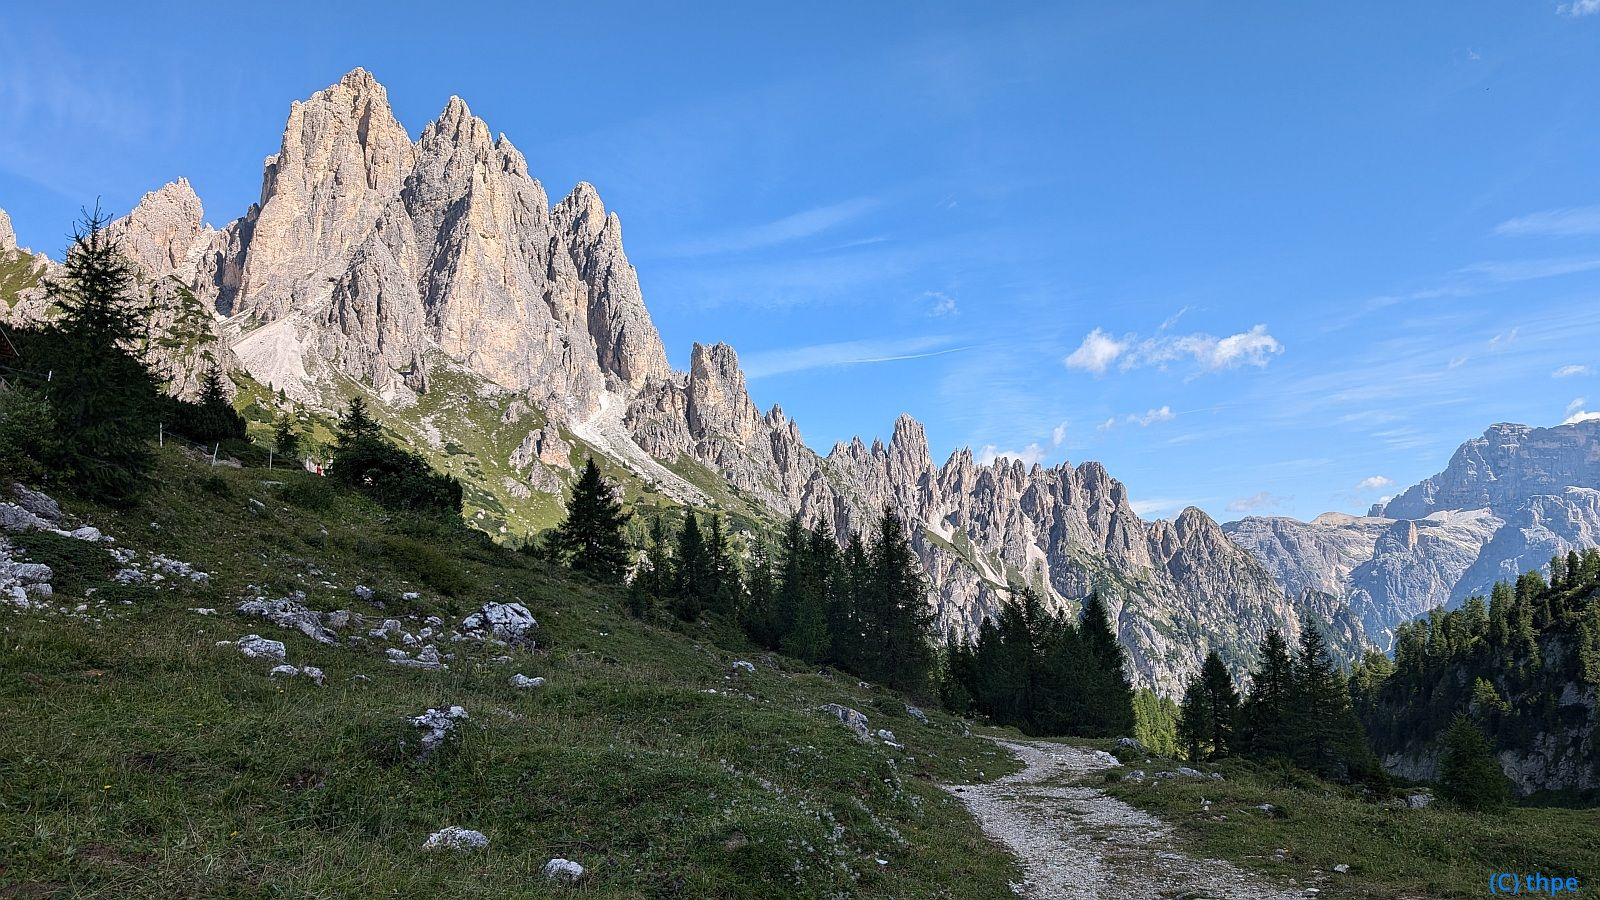
\includegraphics[width=0.6\textwidth,height=\textheight]{mountains.jpg}

}

\caption{\label{fig-mountains}Gebirgslandschaft in den Dolomiten}

\end{figure}%

In Quarto lassen sich externe Bilder und Grafiken im jpg, png oder
pdf-Format einbetten und auch referenzieren
(Abbildung~\ref{fig-mountains}).

Lorem ipsum dolor sit amet, consetetur sadipscing elitr, sed diam nonumy
eirmod tempor invidunt ut labore et dolore magna aliquyam erat, sed diam
voluptua. At vero eos et accusam et justo duo dolores et ea rebum. Stet
clita kasd gubergren, no sea takimata sanctus est Lorem ipsum dolor sit
amet. Lorem ipsum dolor sit amet, consetetur sadipscing elitr, sed diam
nonumy eirmod tempor invidunt ut labore et dolore magna aliquyam erat,
sed diam voluptua. At vero eos et accusam et justo duo dolores et ea
rebum. Stet clita kasd gubergren, no sea takimata sanctus est Lorem
ipsum dolor sit amet. Lorem ipsum dolor sit amet, consetetur sadipscing
elitr, sed diam nonumy eirmod tempor invidunt ut labore et dolore magna
aliquyam erat, sed diam voluptua. At vero eos et accusam et justo duo
dolores et ea rebum. Stet clita kasd gubergren, no sea takimata sanctus
est Lorem ipsum dolor sit amet.

Lorem ipsum dolor sit amet, consetetur sadipscing elitr, sed diam nonumy
eirmod tempor invidunt ut labore et dolore magna aliquyam erat, sed diam
voluptua. At vero eos et accusam et justo duo dolores et ea rebum. Stet
clita kasd gubergren, no sea takimata sanctus est Lorem ipsum dolor sit
amet. Lorem ipsum dolor sit amet, consetetur sadipscing elitr, sed diam
nonumy eirmod tempor invidunt ut labore et dolore magna aliquyam erat,
sed diam voluptua. At vero eos et accusam et justo duo dolores et ea
rebum. Stet clita kasd gubergren, no sea takimata sanctus est Lorem
ipsum dolor sit amet. Lorem ipsum dolor sit amet, consetetur sadipscing
elitr, sed diam nonumy eirmod tempor invidunt ut labore et dolore magna
aliquyam erat, sed diam voluptua. At vero eos et accusam et justo duo
dolores et ea rebum. Stet clita kasd gubergren, no sea takimata sanctus
est Lorem ipsum dolor sit amet.

Lorem ipsum dolor sit amet, consetetur sadipscing elitr, sed diam nonumy
eirmod tempor invidunt ut labore et dolore magna aliquyam erat, sed diam
voluptua. At vero eos et accusam et justo duo dolores et ea rebum. Stet
clita kasd gubergren, no sea takimata sanctus est Lorem ipsum dolor sit
amet. Lorem ipsum dolor sit amet, consetetur sadipscing elitr, sed diam
nonumy eirmod tempor invidunt ut labore et dolore magna aliquyam erat,
sed diam voluptua. At vero eos et accusam et justo duo dolores et ea
rebum. Stet clita kasd gubergren, no sea takimata sanctus est Lorem
ipsum dolor sit amet. Lorem ipsum dolor sit amet, consetetur sadipscing
elitr, sed diam nonumy eirmod tempor invidunt ut labore et dolore magna
aliquyam erat, sed diam voluptua. At vero eos et accusam et justo duo
dolores et ea rebum. Stet clita kasd gubergren, no sea takimata sanctus
est Lorem ipsum dolor sit amet.

Lorem ipsum dolor sit amet, consetetur sadipscing elitr, sed diam nonumy
eirmod tempor invidunt ut labore et dolore magna aliquyam erat, sed diam
voluptua. At vero eos et accusam et justo duo dolores et ea rebum. Stet
clita kasd gubergren, no sea takimata sanctus est Lorem ipsum dolor sit
amet. Lorem ipsum dolor sit amet, consetetur sadipscing elitr, sed diam
nonumy eirmod tempor invidunt ut labore et dolore magna aliquyam erat,
sed diam voluptua. At vero eos et accusam et justo duo dolores et ea
rebum. Stet clita kasd gubergren, no sea takimata sanctus est Lorem
ipsum dolor sit amet. Lorem ipsum dolor sit amet, consetetur sadipscing
elitr, sed diam nonumy eirmod tempor invidunt ut labore et dolore magna
aliquyam erat, sed diam voluptua. At vero eos et accusam et justo duo
dolores et ea rebum. Stet clita kasd gubergren, no sea takimata sanctus
est Lorem ipsum dolor sit amet.

\begin{figure}

\centering{

\includegraphics{quarto-tudscr_files/figure-pdf/fig-histogram-1.pdf}

}

\caption[1000 Zufallszahlen]{\label{fig-histogram}Histogramm aus 1000
standardnormalverteilten Zufallszahlen}

\end{figure}%

Lorem ipsum dolor sit amet, consetetur sadipscing elitr, sed diam nonumy
eirmod tempor invidunt ut labore et dolore magna aliquyam erat, sed diam
voluptua. At vero eos et accusam et justo duo dolores et ea rebum. Stet
clita kasd gubergren, no sea takimata sanctus est Lorem ipsum dolor sit
amet. Lorem ipsum dolor sit amet, consetetur sadipscing elitr, sed diam
nonumy eirmod tempor invidunt ut labore et dolore magna aliquyam erat,
sed diam voluptua. At vero eos et accusam et justo duo dolores et ea
rebum. Stet clita kasd gubergren, no sea takimata sanctus est Lorem
ipsum dolor sit amet. Lorem ipsum dolor sit amet, consetetur sadipscing
elitr, sed diam nonumy eirmod tempor invidunt ut labore et dolore magna
aliquyam erat, sed diam voluptua. At vero eos et accusam et justo duo
dolores et ea rebum. Stet clita kasd gubergren, no sea takimata sanctus
est Lorem ipsum dolor sit amet.

\chapter{Diskussion}\label{diskussion}

Duis autem vel eum iriure dolor in hendrerit in vulputate velit esse
molestie consequat, vel illum dolore eu feugiat nulla facilisis at vero
eros et accumsan et iusto odio dignissim qui blandit praesent luptatum
zzril delenit augue duis dolore te feugait nulla facilisi.

\chapter*{Danksagung}\label{danksagung}
\addcontentsline{toc}{chapter}{Danksagung}

Hier ist es besonders wichtig, Kooperations- und Praxispartnern zu
danken, von denen man Unterstützung oder Daten erhalten hat. Bei
Drittmittelfinanzierung muss der Fördermittelgeber und das
Förderkennzeichen angegeben werden.

\chapter*{Selbständigkeitserklärung}\label{selbstuxe4ndigkeitserkluxe4rung}
\addcontentsline{toc}{chapter}{Selbständigkeitserklärung}

Bei Prüfungs- und Abschlussarbeiten muss im Regelfall eine
Selbständigkeitserklärung angegeben werden.

\chapter*{Literatur}\label{literatur}
\addcontentsline{toc}{chapter}{Literatur}

\phantomsection\label{refs}
\begin{CSLReferences}{1}{0}
\bibitem[\citeproctext]{ref-Hanisch2022}
Hanisch, F. (2022). \emph{Ein LATEX-Bundle für Dokumente im Corporate
Design der Technischen Universität Dresden. Benutzerhandbuch.} TU
Dresden. \url{https://tug.org/docs/latex/tudscr/tudscr.pdf}

\bibitem[\citeproctext]{ref-latex-manual}
Lamport, L. (2005). \emph{The LaTeX Manual. 2nd edition.} {American
Mathematical Society}.

\bibitem[\citeproctext]{ref-RStudio2024}
Posit Team. (2024). \emph{Rstudio: Integrated Development Environment
for R}. Posit Software, PBC. \url{https://www.posit.co/}

\bibitem[\citeproctext]{ref-RCore2024}
R Core Team. (2024). \emph{R: A Language and Environment for Statistical
Computing}. R Foundation for Statistical Computing.
\url{https://www.R-project.org/}

\bibitem[\citeproctext]{ref-Quarto2024}
RStudio Team. (2024). \emph{Quarto: A Publishing Platform} (Version
1.4.554). \url{https://quarto.org}

\end{CSLReferences}



\end{document}
